\scanpage{93}
\mspage{14}
action sur \deleted{$H_{x_i,x_0}$} le système $(\Pi_0,H_{x_i,x_0},\underbrace{\Pi_0/\Pi'_0}_{\deleted{\unsure{esp|espace}}})$ où on fait opérer $\Theta$ sur $\Pi_0,H_{(x_i,x_0)}$ par son action sur $\mathcal C$, et sur $\Pi_0/\Pi'_0$ via l'action sur $\Pi_0$, qui passe au quotient d'après la \deleted{hypothèse} \inserted{condition} \deleted{dite} envisagée. L'action \deleted{prolong} remontée \inserted{$\unsure{\widetilde\Theta|\Theta'}$ de $\Theta$} \deleted{est} sur $\widetilde{\mathcal C}$ est donc unique. Pour qu'il existe une action de $\Theta^{*}$ sur $\mathcal C'$ qui soit compatible avec $\mathcal C'-\mathcal C$, il f. et s. que la condition précédente soit satisfaite, et que \uline{de plus} $\operatorname{Ob}\mathcal C'\subset\operatorname{Ob}\mathcal C$ soit stable sous \deleted{cette} l'action de $\widetilde\Theta$.

Dans le cas où on ne suppose pas que l'on \deleted{dispose de} \inserted{donne} un $x'_0\in\operatorname{Ob}\mathcal C'$ dont on exige qu'il soit fixe par $\Theta$, on considère la fibre \inserted{$E_0=$} $\widetilde{\mathcal C}_{x_0}$, qui est un $\Pi_0$-ensemble \deleted{\unsure{un}} homogène, et on note que les façons de remonter $\Theta$ en une action \inserted{$\widetilde\Theta$} dans $\widetilde{\mathcal C}$ correspondent \deleted{\unsure{aux}} exactement aux façons de remonter $\Theta$ en une action de $\widetilde\Theta_0$ sur $E_0$, \deleted{\unsure{comment|convenant}} soit compatible avec l'action sur $\Pi_0$, i.e. satisfaisant
\margin{mais on suppose tjrs un $x_0$ fixe sous $\Theta$}
\figure{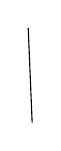
\begin{tikzpicture}\draw(0,0)--(-.05,1.2);\end{tikzpicture}}
\margin{Ceci vaut sans supposer $\widetilde{\mathcal C}$ connexe --- mais la traduction plus bas en termes de $\Pi'_0\subset\Pi_0$ dépend de la condition de connexité.\ldots Cf plus bas le cas où on a un \unsure{s-grp} plein $\mathcal C$ connexe.}
\[
\tag{46}\widetilde\Theta_0(g.x^{\deleted{\unsure{0}}\prime})=\Theta(g)\widetilde\Theta_0(x')
\]
--- \deleted{elle correspond} \inserted{une telle action} est connue quand on connaît, pour \uline{un} $x'_0$ fixé de $E_0=\operatorname{Ob}\widetilde{\mathcal C}_{x_0}$, son transformé par $\widetilde\Theta_0$, la formule (46) donnant tous les autres \inserted{$\widetilde\Theta_0(x')$, \deleted{puisque $\unsure{x'\in E_0}$} $\unsure{\mathrm{pr}|\forall}\,x'\in E_0$}. En termes
\margin{92}
